\documentclass[border=1cm]{standalone}

\usepackage{tikz}
\usetikzlibrary{arrows,calc,intersections}
\begin{document}

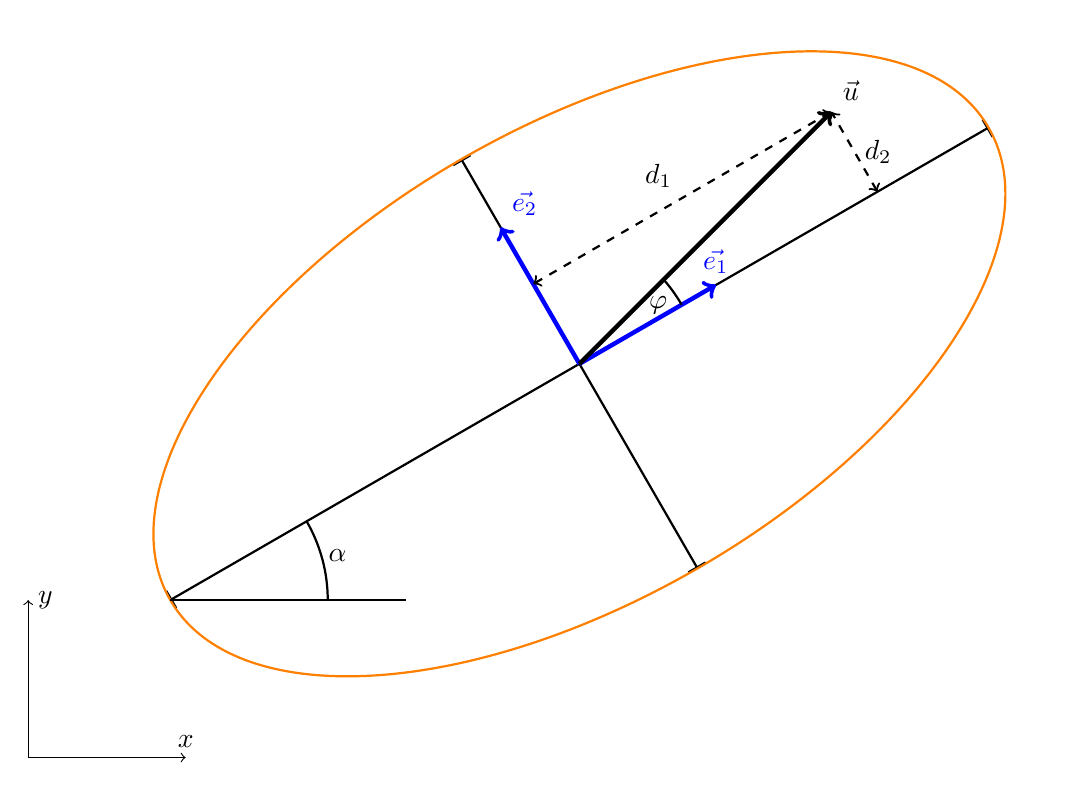
\begin{tikzpicture}[scale=2]
    % Define the angle
    \def\uhel{30}

    % Draw the line segment with length 6 in the direction of angle \uhel
    \draw[|-|, thick, ] ({-3*cos(\uhel)}, {-3*sin(\uhel)}) -- ({3*cos(\uhel)}, {3*sin(\uhel)}) ;

    % Draw the line segment with length 6 in the direction of angle \uhel
    \def\delka{1.5}
    \draw[|-|, thick, ] ({-\delka*cos(\uhel+90)}, {-\delka*sin(\uhel+90)}) -- ({\delka*cos(\uhel+90)}, {\delka*sin(\uhel+90)}) ;



    % Draw the unit vector in the direction of angle \uhel
    \draw[->, ultra thick, blue] (0,0) -- ({cos(\uhel)}, {sin(\uhel)}) node[anchor=south] {$\vec{e_1}$};

    \draw[->, ultra thick, blue] (0,0) -- ({cos(\uhel+90)}, {sin(\uhel+90)}) node[anchor=south west] {$\vec{e_2}$};

    \draw[->, ultra thick] (0,0) -- (1.6,1.6) node[anchor=south west] {$\vec u$};

    \pgfmathsetmacro{\prumet}{1.6*cos(\uhel+90)+1.6*sin(\uhel+90)}
    \draw[<->, thick, dashed] ({\prumet*cos(\uhel+90)}, {\prumet*sin(\uhel+90)}) --  node[anchor=south east] {$d_1$} (1.6,1.6);

    \pgfmathsetmacro{\prumet}{1.6*cos(\uhel)+1.6*sin(\uhel)}
    \draw[<->, thick, dashed] ({\prumet*cos(\uhel)}, {\prumet*sin(\uhel)}) --  node[anchor=west] {$d_2$} (1.6,1.6);

    \draw[thick] ({0.75*cos(\uhel)},{0.75*sin(\uhel)}) 
      node[shift={(-0.3,0)}]{$\varphi$} arc[start angle=\uhel, end angle=\uhel+12, radius=1];
    


    \begin{scope}[shift={({-3*cos(\uhel)}, {-3*sin(\uhel)})}]
    \draw[thick] (1,0) arc[start angle=0, end angle=\uhel, radius=1];
    \node at ({1.1*cos(\uhel/2)}, {1.1*sin(\uhel/2)}) {$\alpha$};
    \end{scope}
    
    % Nastavení elipsy
    \def\polosA{3}   % Délka hlavní poloosy
    \def\polosB{1.5} % Délka vedlejší poloosy
    \def\uhel{30}    % Úhel otočení

    % Kreslení elipsy
    \draw[thick, orange, rotate=\uhel] (0,0) ellipse (\polosA cm and \polosB cm);

    \draw[] ({-3*cos(\uhel)}, {-3*sin(\uhel)}) -- ({-3*cos(\uhel)+1.5}, {-3*sin(\uhel)});

    
    \begin{scope}[shift={(-3.5,-2.5)}]
    \draw[->](0,0)--(1,0) node[above] {$x$};
    \draw[->](0,0)--(0,1) node[right] {$y$};
    \end{scope}
\end{tikzpicture}

\end{document}